\documentclass[14pt]{extarticle}
% \documentclass[14pt]{article}

% \usepackage[style=authoryear,maxbibnames=9,maxcitenames=2,uniquelist=false,backend=biber,doi=false,url=false]{biblatex}
% \addbibresource{$BIB} % bibtex location
% \renewcommand*{\nameyeardelim}{\addcomma\space} % have comma in parencite
\usepackage{natbib}

\usepackage{xcolor}
\usepackage{amsmath}
\newcommand{\tuple}[1]{ \langle #1 \rangle }
%\usepackage{automata}
\usepackage{times}
\usepackage{ltablex}
\usepackage{tasks}

%%%%%% Template
\usepackage{hyperref}
\hypersetup{colorlinks=true,allcolors=blue}

\usepackage{vmargin}
\setpapersize{USletter}
\setmarginsrb{1.0in}{1.0in}{1.0in}{0.6in}{0pt}{0pt}{0pt}{0.4in}

% HOW TO USE THE ABOVE:
%\setmarginsrb{leftmargin}{topmargin}{rightmargin}{bottommargin}{headheight}{headsep}{footheight}{footskip}
%\raggedbottom
% paragraphs indent & skip:
\parindent  0.3cm
\parskip    -0.01cm

\usepackage{tikz}
\usetikzlibrary{backgrounds}

% hyphenation:
% \hyphenpenalty=10000 % no hyphen
% \exhyphenpenalty=10000 % no hyphen
\sloppy

% notes-style paragraph spacing and indentation:
\usepackage{parskip}
\setlength{\parindent}{0cm}

% let derivations break across pages
\allowdisplaybreaks

\newcommand{\orange}[1]{\textcolor{orange}{#1}}
\newcommand{\blue}[1]{\textcolor{blue}{#1}}
\newcommand{\red}[1]{\textcolor{red}{#1}}
\newcommand{\freq}[1]{{\bf \sf F}(#1)}
\newcommand{\datafreq}[2]{{{\bf \sf F}_{#1}(#2)}}

\def\qqquad{\quad\qquad}
\def\qqqquad{\qquad\qquad}

%%%%%%%%%%%%%%%%%%%%%%%%%%%%%%%%%%%%%%%%%%%%%%%%%%%%%%%%%%%%%%%%%%%%%%%%%%%%%%%%
%%%%%%%%%%%%%%%%%%%%%%%%%%%%%%%%%%%%%%%%%%%%%%%%%%%%%%%%%%%%%%%%%%%%%%%%%%%%%%%%

% fill-in-blank question style, found in https://tex.stackexchange.com/a/505089

\usepackage{ifthen}
\usepackage{tocloft}
\usepackage{exercise}
% \usepackage{xcolor}

% Set the Show Answers Boolean
\newboolean{showAns}
\setboolean{showAns}{false}
\newcommand{\showAns}{\setboolean{showAns}{true}}

% The length of the Answer line
\newlength{\answerlength}
\newcommand{\anslen}[1]{\settowidth{\answerlength}{#1}}

% ans command that indicates space for an answer or shows the answer in red
\newcommand{\ans}[1]{\settowidth{\answerlength}{\hspace{2ex}#1\hspace{2ex}}%
    \ifthenelse{\boolean{showAns}}%
        {\textcolor{red}{\underline{\hspace{2ex}#1\hspace{2ex}}}}%
        {\underline{\hspace{\answerlength}}}}%

\newcommand{\details}[1]{\settowidth{\answerlength}{#1}%
    \ifthenelse{\boolean{showAns}}%
        {\\ \textcolor{blue}{#1}}%
        {}}%

% Formatting how multiple choices Questions are formated.
\settasks{label=(\Alph*), label-width=30pt}


% Some commands for the Exercise Question package
\renewcommand{\QuestionNB}{\Large\protect\textcircled{\small\bfseries\arabic{Question}}\ }
\renewcommand{\ExerciseHeader}{} %no header
\renewcommand{\QuestionBefore}{3ex} %Space above each Q
\setlength{\QuestionIndent}{8pt} % Indent after Q number


% To create the list of answers with tocloft...
\newcommand{\listanswername}{Answers}
\newlistof[Question]{answer}{Answers}{\listanswername}

% Creates a TOC for Answers
\newcounter{prevQ}
\newcommand{\answer}[1]{\refstepcounter{answer}%
\ans{#1}%
\ifnum\theQuestion=\theprevQ%
        \addcontentsline{Answers}{answer}{\protect\numberline{}#1}% don't include the Q number
        \else%
        \addcontentsline{Answers}{answer}{\protect\numberline{\theQuestion}#1}%
        \setcounter{prevQ}{\value{Question}}%
        \fi%
        }%

% \hyphenpenalty=10000 % no hyphen
% \exhyphenpenalty=10000 % no hyphen
\sloppy              % hyphen

\newcommand{\HRule}{\rule{\linewidth}{0.5mm}}
\newcommand{\Hrule}{\rule{\linewidth}{0.3mm}}

%tocloft formatting listofanswers
\renewcommand{\cftAnswerstitlefont}{\bfseries\large}
\renewcommand{\cftanswerdotsep}{\cftnodots}
\cftpagenumbersoff{answer}
\addtolength{\cftanswernumwidth}{10pt}

\makeatletter% since there's an at-sign (@) in the command name
\renewcommand{\@maketitle}{%
  \parindent=0pt% don't indent paragraphs in the title block
  \centering
  {\Large \bfseries\textsc{\@title}} \\
  \vspace{5pt}
  {\large \textit{\@author}} \\
  \HRule \\
  \vspace{1em}
}
\makeatother% resets the meaning of the at-sign (@)

\title{ECON 2002.01 Problem Set 9}
\author{Unit 15 \\
  \vspace{5pt}
    Hui-Jun Chen}


%%%%%%%%%%%%%%%%%%%%%%%%%%%%%%%%%%%%%%%%%%%%%%%%%%%%%%%%%%%%%%%%%%%%%%%%%%%%%%%%
%%%%%%%%%%%%%%%%%%%%%%%%%%%%%%%%%%%%%%%%%%%%%%%%%%%%%%%%%%%%%%%%%%%%%%%%%%%%%%%%
\begin{document}

\maketitle

\showAns
\listofanswer

    % 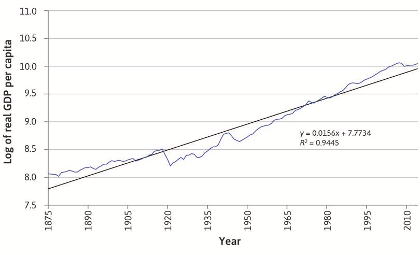
\includegraphics[width=\textwidth]{../QuestionBankImage/OUP-U13-Q04-01.png}

\begin{Exercise}



\Question (OUP-U15-Q2)
Which of the following is a definite consequence of a high inflation rate?
\answer{D}
\begin{tasks}(1)
    \task It reduces everyone’s real wealth and real income.
        \details{Inflation is unlikely to reduce everyone’s real income and wealth. The first depends upon the composition of one’s wealth. Some assets, especially real assets, can rise in price along with inflation. In the UK, house prices have often risen faster than inflation. Likewise, protecting one’s real income from inflation depends on one’s ability to bargain for a money wage increase. Depending on these conditions, some people will be losers but some may possibly benefit from inflation. The fact that who wins and who loses is something of a lottery is sometimes given as a reason for objecting to inflation.}
    \task It makes borrowing more expensive.
        \details{The cost of borrowing depends upon the real rate of interest, which is the nominal rate minus the rate of inflation. Inflation will make borrowing cheaper if the nominal rate of interest does not adjust sufficiently.}
    \task It makes poor people worse off.
        \details{This is not an ineoutcome. It depends on whether their nominal incomes and their assets keep pace with the rising price level.}
    \task It can distort price signals.
        \details{A change in price is an important signal in market economies. It can signal the need to buy more or less, supply more or less, and so on. If prices are generally rising, it can be difficult to know what an individual price increase means. Does it mean increasing scarcity, in which case some reallocation decision is required, or it is just part of the inflationary process? This can be a serious problem if inflation is running at a high rate, and especially if the rate is frequently changing.}
\end{tasks}




\Question (OUP-U15-Q5)
Imagine that the rate of inflation has been 10 per cent per year for a number of years. The central bank then introduces a ‘tight’ monetary policy and the rate of inflation comes down to 5 per cent per year. This reduction is an example of:
\answer{C}
\begin{tasks}(1)
    \task Deflation.
        \details{Deflation is a situation in which prices are actually falling. That is not the case here. It is the rate of change of prices that is falling.}
    \task Falling prices.
        \details{Falling prices means deflation, which is not the case here.}
    \task Disinflation.
        \details{Correct. Disinflation refers to a situation where inflation (the rate of change of prices) is being reduced.}
    \task Austerity.
        \details{‘Austerity’ is a political term that usually refers to a situation where a tight fiscal policy involves strict limits on or even cuts in public spending. It may be motivated by a need to reduce aggregate demand in order to reduce the rate of inflation. It is the name given to a policy, not to the outcome, and in this example, it is a tight monetary not fiscal policy that is used.}
\end{tasks}



\Question (OUP-U15-Q11)
Suppose that the bargaining power of workers rises relative to that of employers because government legislation improves the security of employment. In terms of the wage-setting/price-setting model shown in the figure:

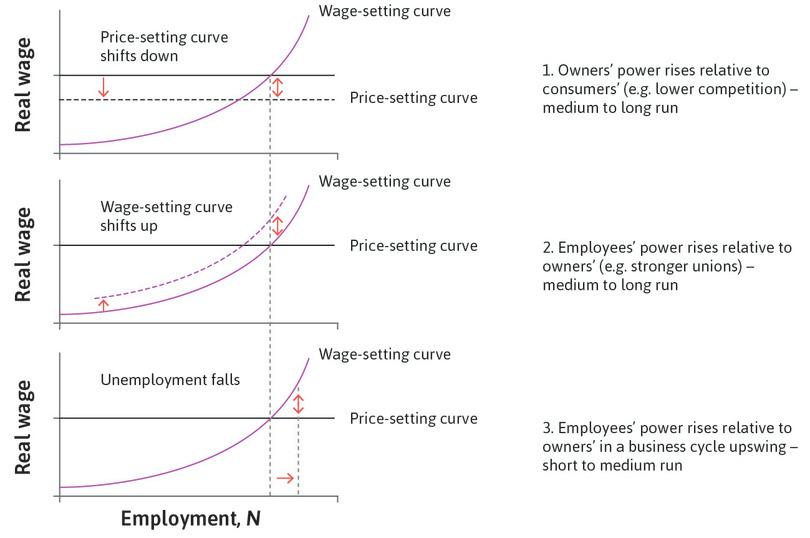
\includegraphics[width=\textwidth]{../QuestionBankImage/OUP-U15-Q11-01.jpg}
\answer{B}
\begin{tasks}(1)
    \task We move along the wage-setting curve, to the right.
        \details{No. A movement along a given wage-setting curve would require a change in the level of employment, since the diagram shows how the workers’ desired real wage varies with the level of employment.}
    \task The wage-setting curve moves up.
        \details{Correct. The wage-setting curve shifts up because the improved security of employment encourages workers to seek higher wages at every level of employment.}
    \task The wage-setting curve moves down.
        \details{No. This would suggest that the legislation encouraged workers to settle for lower wages at every level of employment.}
    \task The wage-setting curve becomes flatter.
        \details{This would suggest that workers were becoming less concerned about higher real wages as employment expands, which is not guaranteed by a rise in their bargaining power.}
\end{tasks}




\Question (OUP-U15-Q17)
The original Phillips curve shown in the figure suggested that the policymaker could choose:
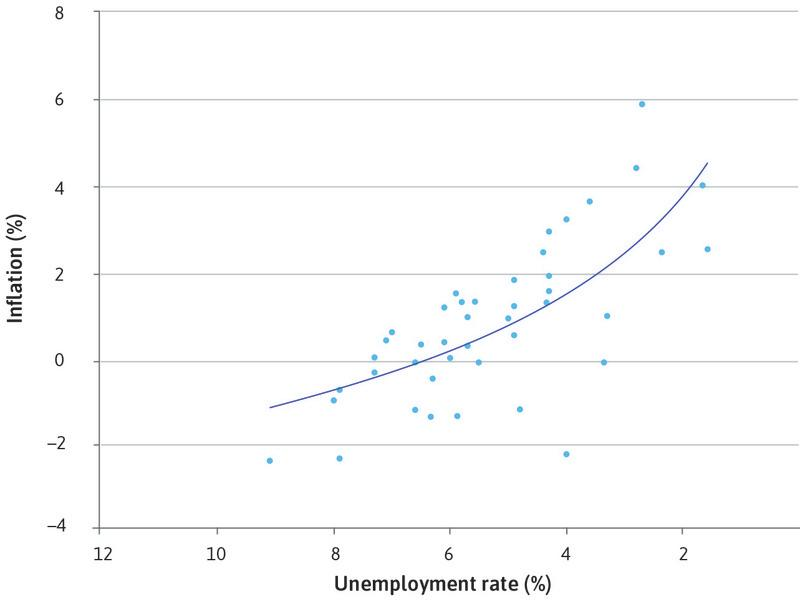
\includegraphics[width=\textwidth]{../QuestionBankImage/OUP-U15-Q17-01.jpg}

\answer{C}
\begin{tasks}(1)
    \task Any preferred level of unemployment and inflation.
        \details{No. The original Phillips curve suggested the policymaker could choose any level of unemployment, but only by accepting the associated rate of inflation.}
    \task Any preferred rate of inflation, for a given level of unemployment.
        \details{Similarly, for a given level of unemployment, the policymaker has to accept the associated rate of inflation.}
    \task A stable combination of inflation and unemployment.
        \details{The important message from the original Phillips curve was that this choice, once made, would be lasting. It need not change unless the policymaker chose a different combination.}
    \task A temporary combination of inflation and unemployment.
        \details{No. It was subsequent developments of the Phillips curve that suggested that these combinations could not be maintained and were only temporary.}
\end{tasks}




\Question (OUP-U15-Q20)
Assume that a bargaining gap remains constant at 1 per cent. The rate of inflation in future years will:
\answer{C}
\begin{tasks}(1)
    \task Remain constant at 1 per cent per year.
        \details{No. If there is a positive bargaining gap, there will be upward pressure on prices. This will be added to any existing rate of inflation, so the rate of inflation must accelerate.}
    \task Remain unchanged.
        \details{No. For the same reason, inflation must be accelerating.}
    \task Accelerate by 1 per cent per year.
        \details{Correct. If the bargaining gap is constant at 1 per cent, this will be added to the rate of inflation each year and so inflation will increase (accelerate) by 1 per cent per year.}
    \task Settle at 1 per cent.
        \details{No. So long as there is a bargaining gap, inflation cannot settle at any level. It must be accelerating or decelerating.}
\end{tasks}



\Question (OUP-U15-Q22)
Assume that the central bank has an inflation target of 2\% per year but inflation is currently running at 4\%. The nominal policy (interest) rate is currently 5\%. The central bank needs to create a negative bargaining gap and estimates that the real policy rate required to achieve this is 3\%. Consequently it needs to set the nominal policy rate at:
\answer{B}
\begin{tasks}(1)
    \task 6\%.
        \details{No. If inflation is running at 4\% and the real rate needs to be 3\%, then according to the Fisher equation, the nominal rate needs to be 4\% + 3\% = 7\%.}
    \task 7\%.
        \details{According to the Fisher equation, 7\% is the required nominal rate.}
    \task 8\%.
        \details{No. If inflation is running at 4\% and the real rate needs to be 3\%, then according to the Fisher equation, the nominal rate needs to be 4\% + 3\% = 7\%.}
    \task 4\%.
        \details{No. The required rate is 4 + 3 = 7\%.}
\end{tasks}



\Question (OUP-U15-Q25)
It is often said that independent central banks are more likely to run a successful monetary policy than governments because their commitment to low inflation is more ‘credible’ than government promises. One reason for this is that:
\answer{D}
\begin{tasks}(1)
    \task Independent central banks are better at economic forecasting.
        \details{There is no reason to suppose that independent central banks are systematically better at forecasting than ministries of finance or private firms.}
    \task People who work in central banks have a strong dislike of inflation.
        \details{It may be possible that people who occupy senior positions in central banks are more inflation-averse than politicians or even than members of the public. If this is true, then they may be tempted to run monetary policy in their own interests and therefore with a low inflation bias. But there is no evidence for this and it is difficult to see why there would be this systematic bias.}
    \task Central banks can set interest rates.
        \details{It is true that central banks can set interest rates. In fact it is only a central bank that can impose a particular interest rate on the financial system. But the power to set the interest rate is a different issue from deciding what rate to set. It is the latter that has been moved from governments to independent central banks in recent years. It would be perfectly possible to return the decision-making to government, even though the central bank would still have to impose the rate.}
    \task Central banks are less subject to political pressures (e.g. for lower unemployment) than governments.
        \details{The argument for putting the decision in the hands of an independent central bank is based upon the view that central banks face fewer conflicts of interest, because they are not subject to political pressures. If inflation requires a very high (and unpopular) rate of interest, this is less of a problem for central banks than for governments whose electors may be more concerned about jobs.}
\end{tasks}



\Question (ECO-U15-Q5)
See Figure 15.4d for diagrams of the labour market model, the Phillips curve, and the multiplier model of aggregate demand. The unemployment rates and the bargaining gaps at different states of the economy are shown. Based on this information, which of the following statements is correct?
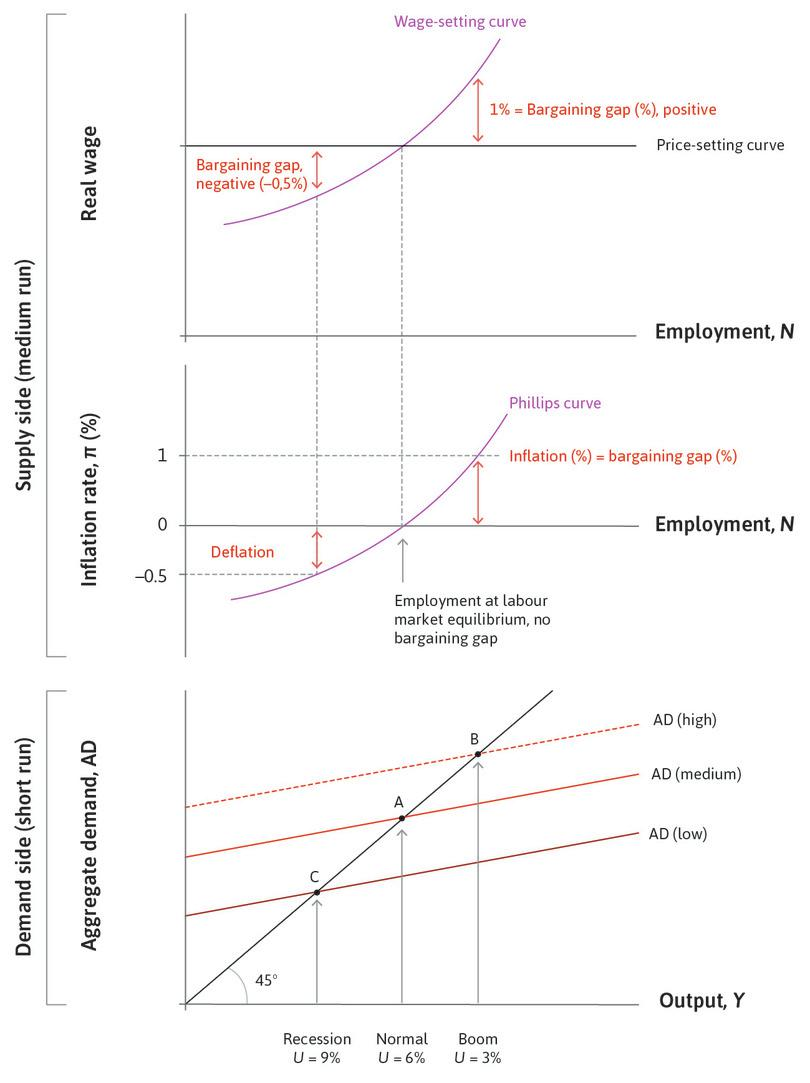
\includegraphics[width=\textwidth]{../QuestionBankImage/ECO-U15-Q5-01.jpg}
\answer{B}
\begin{tasks}(1)
    \task There is no inflation when the unemployment rate is zero.
        \details{There is always a positive rate of unemployment in the labour market model (see Unit 9). If U is below 3\%, then there would be an even larger positive bargaining gap than with U = 3 and even higher inflation. Inflation is zero in the diagram only when the unemployment rate is 6\%.}
    \task In the boom shown, the upward shift in the aggregate demand curve reduces the unemployment rate, which in turn creates a bargaining gap of 1\%.
        \details{At point B unemployment is below the labour market equilibrium, creating a positive bargaining gap.}
    \task In the recession shown, the downward shift in the aggregate demand curve increases the unemployment rate, which in turn creates a bargaining gap of 0.5\%.
        \details{The bargaining gap created as a result of the recession is –0.5\%, which is negative.}
    \task The resulting Phillips curve shows a positive correlation between the unemployment rate and inflation rate.
        \details{The Phillips curve shows a positive correlation between employment and the inflation rate, which means a negative correlation between the unemployment rate and the inflation rate.}
\end{tasks}



\Question (OUP-U15-Q18)
The main weakness of the original Phillips curve is that it ignored:
\answer{D}
\begin{tasks}(1)
    \task Time.
        \details{It didn’t ignore time; Phillips used data from 1861 to 1957. The problem was that the data for this period was misleading as a guide to the post-1957 period.}
    \task Household preferences.
        \details{There was no issue regarding household preferences.}
    \task Policymaker preferences.
        \details{There was no problem with regard to policymaker preferences, except that the original Phillips curve suggested that the feasible combinations were durable.}
    \task Expectations.
        \details{Correct. The problem was expectations. The original Phillips curve was based upon data drawn from a period when inflation was generally very low (excluding the two world wars). Therefore, in the process of wage bargaining, the future expected rate of inflation was not a major factor. In more inflationary times (1960 onwards) it was inevitable that whatever the level of unemployment and the size of the bargaining gap, workers would also be trying to take account of what they expected inflation to be, guided by the most recent rate.}
\end{tasks}



\Question (OUP-U15-Q25)
It is often said that independent central banks are more likely to run a successful monetary policy than governments because their commitment to low inflation is more ‘credible’ than government promises. One reason for this is that:
\answer{D}
\begin{tasks}(1)
    \task Independent central banks are better at economic forecasting.
        \details{There is no reason to suppose that independent central banks are systematically better at forecasting than ministries of finance or private firms.}
    \task People who work in central banks have a strong dislike of inflation.
        \details{It may be possible that people who occupy senior positions in central banks are more inflation-averse than politicians or even than members of the public. If this is true, then they may be tempted to run monetary policy in their own interests and therefore with a low inflation bias. But there is no evidence for this and it is difficult to see why there would be this systematic bias.}
    \task Central banks can set interest rates.
        \details{It is true that central banks can set interest rates. In fact it is only a central bank that can impose a particular interest rate on the financial system. But the power to set the interest rate is a different issue from deciding what rate to set. It is the latter that has been moved from governments to independent central banks in recent years. It would be perfectly possible to return the decision-making to government, even though the central bank would still have to impose the rate.}
    \task Central banks are less subject to political pressures (e.g. for lower unemployment) than governments.
        \details{The argument for putting the decision in the hands of an independent central bank is based upon the view that central banks face fewer conflicts of interest, because they are not subject to political pressures. If inflation requires a very high (and unpopular) rate of interest, this is less of a problem for central banks than for governments whose electors may be more concerned about jobs.}
\end{tasks}

\end{Exercise}

\end{document}
